\section{Korisničko sučelje}
Svaka igra mora imati svoje korisničko sučelje (\emph{eng. User Interface UI}) gdje će korisnici moći mijenjati pojedine opcije igre. Unity za ovo pruža poseban igrajući objekt koji se zove platno (\emph{eng. Canvas}). Ukoliko platno već nije izrađeno, onda prilikom izrade teksta za sučelje će unity sam napraviti i platno i tekst kao dijete platna. Dakle sve objekte koji pripadaju korisničkom sučelju moraju biti dijete platna u hijerarhiji.
\subsection{Platno}
Sva platna su ustvari 2D objekti kojima je dodana dubina samo boljeg prikaza u 3D prostoru. Prebacivanjem u 3D pogled će se moći vidjeti da platna izgledaju kao običan list papira na kojima je nekakav tekst, botun ili slika. Igrajući objekti koji su dio platna će se prikazivati prema njihovom položaju u hijerarhiji. Dakle ako imamo više igrajućih objekata, onda će se prvo nacrtati prvo dijete i svi igrajući objekti koji njegova djeca, zatim će drugo dijete i tako dalje. Platno također ima različite modove izrade (\emph{eng. Render modes}).
\subsubsection{Raspored elemenata}
Pod rasporedom (\emph{eng. Layout}) se misli pozicija pojedinih elemenata unutar platna. Dakle dimenzije i odnos prema drugim elementima. Sidrišta (\emph{eng. Anchors}) imaju jako veliku pri odnosu pojedinih elemata, a o njima će više biti rečenu u nastavaku. Veličina platna se može mijenjati korištenjem alata \emph{Rect Transform}, koji se ponaša kao pravokutnik. Uglavnom se koristi za 2D objekte, ali naravno može i za 3D objekte. Isto tako se može mijenjati pozicija elemenata jednostavnim označavanjem i povlačenjem na željenu lokaciju. Potrebno je razlikovati prilikom mijenjanja veličine objekta da postoje dvije različite transformacije koje se čine jednake. Ako se koristi alat \emph{Rect Tool} označen objekt tada mijenja svoju veličinu (\emph{eng. Scale}), a ako je selektiran \emph{Rect Transform} mijenjaju se dimenzije objekta (širina i visina). 
\newpage
\subsubsection{Sidrišta}
Sidrišta su četiri trokutasta elementa koja definiraju točku od koje će se kretati elementi i koju će pratiti za promjene. Zanimljiva funkcionalnost koja omogućavaju da element mijenja dimenzije ovisno o promjeni dimenzija elemenata na koji je pridružen, ako ujedno i je pridružen. Moguće je na drugi element postaviti da sidrište prati visinu odabranog elementa, te će se trenutni element mijenjati relativno s obzirom na pridruženi. Na slici \ref{fig:sidriste} je moguće vidjeti tekstualni element kojemu je sidrište postavljeno da prati gornji desni kut roditelja. Na ovaj način će se tekst uvijek pomicati relativno sa gornjim desnim kutom.
\begin{figure}[h]
	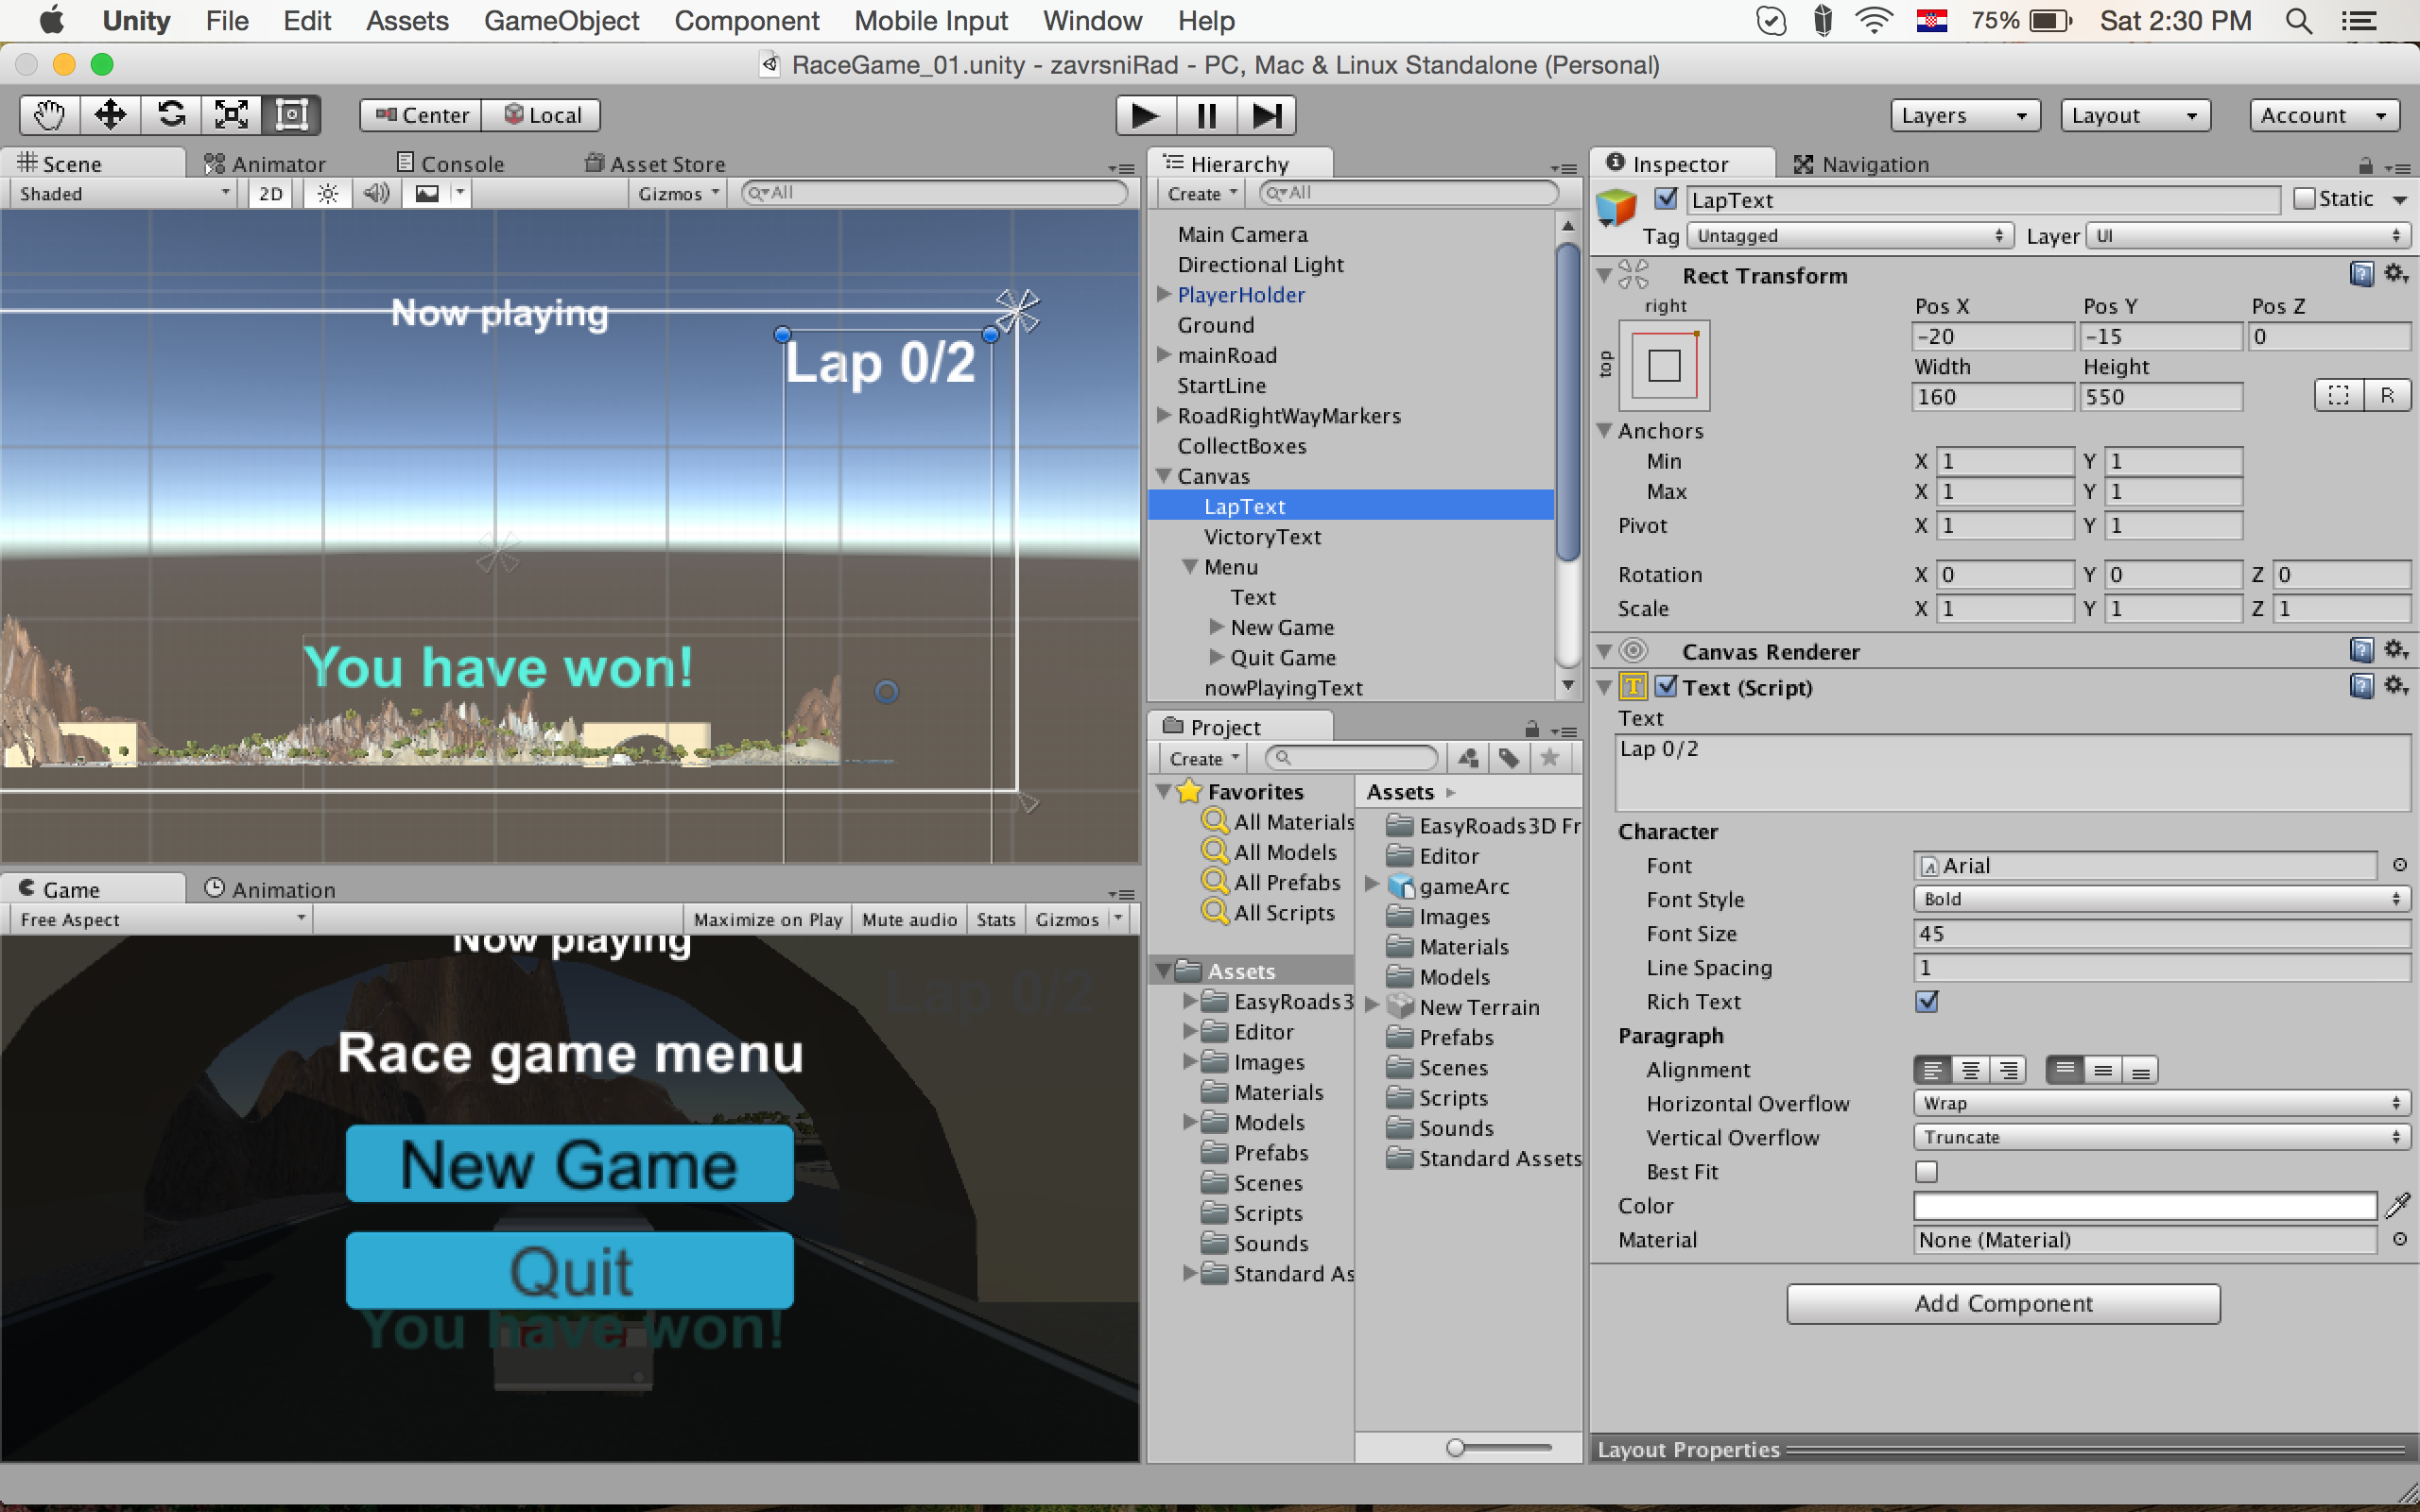
\includegraphics[width=12.5cm, height=8cm]{sidriste.png}
	\centering
	\caption{Sidrište}
	\label{fig:sidriste}
\end{figure}
\newline
Sa desne strane je moguće vidjeti sve komponente koje ima element, te standardne opcije kao što su x, y i z transformacija unutar roditelja, visina i širina, minimalna i maksimalna vrijednost sidrišta i veličina. Tekstu možemo definirati oblik, veličinu, poravnavanje i boju.
\newpage

\subsubsection{Modovi izrade}
Postoje dvije glavne podjele ovih modova:
\begin{itemize} 
	\item Pozicija zaslona (\emph{eng. Screen Space}) - platno se pozicionira prema poziciji zaslona. 
		\begin{itemize}
			\item Prekriti (\emph{eng. Overlay}) - svi objekti se izrađuju na platnu, te mijenjaju svoju veličinu ovisno o veličini platna
			\item Kamera - svi objekti se izrađuju ovisno o postavkama kamere. Ako se na kameri promijeni perspektiva, tada će se i sami izgled sučelja mijenjati ovisno o udaljenosti, kutu, te svim ostalim parametrima koji su postavljeni.
		\end{itemize}
	\item Pozicija svijeta (\emph{eng. World Space}) - platno se ponaša kao svaki drugi igrajući objekt. Moći će se postaviti u pozadini iza nekih drugih igrajućih objekata ili slično. Primjer bi bio prikaz teksta koji se mijenja na nekakvom računalu.
\end{itemize}

\subsection{Glavni izbornik}
Glavni izbornik se sastoji od tri igrajuća objekta, jednog teksta i dva botuna. Izborniku je pridružena i skripta koja kontrolira prikaz i funkcionalnost botuna. Koristi se od unity-a ugrađena funkcionalnost za pozivanja metoda unutar skripte. Svaki botun ima okidač na klik, te se samo treba postaviti metoda koja se želi pozvati. U igri su to dvije metode započmi novu igru (\emph{StartNewGame}) i izađi iz igre (\emph{StartNewGame}). Izgled izbornika se može vidjeti na slici \ref{fig:glavniIzbornik}.
\begin{figure}[h]
	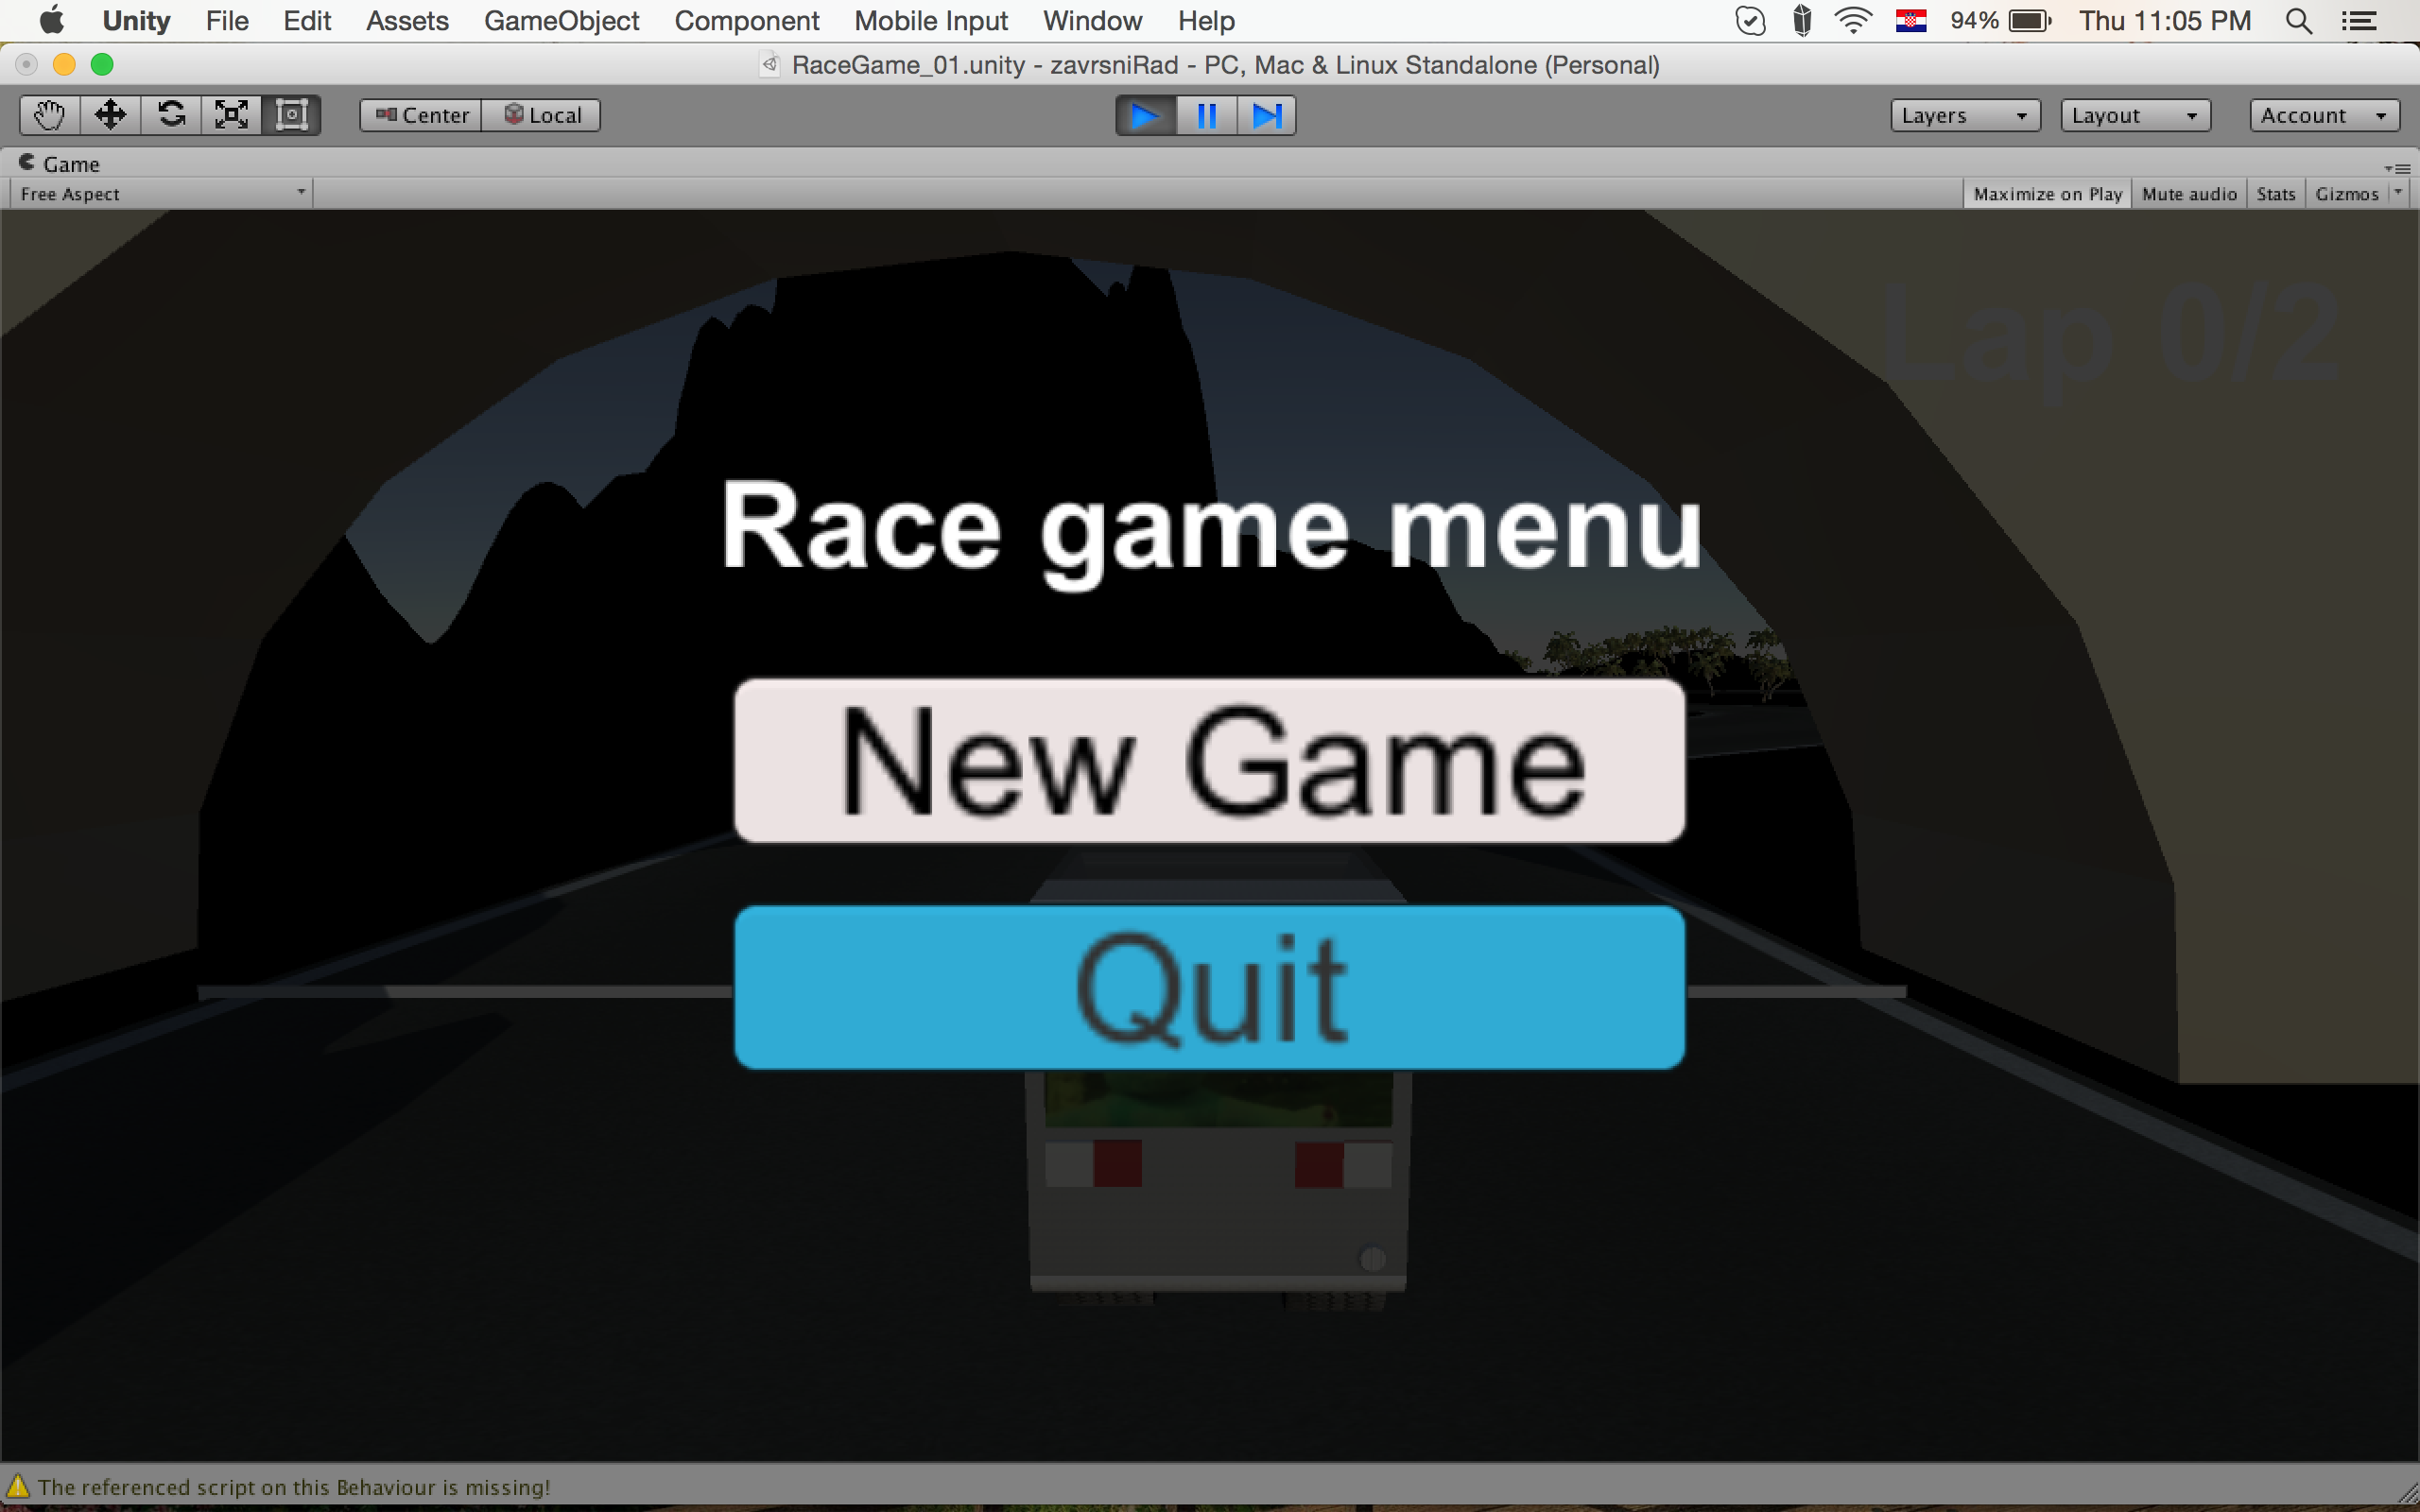
\includegraphics[width=12.5cm, height=8cm]{glavni_izbornik.png}
	\centering
	\caption{Glavni izbornik}
	\label{fig:glavniIzbornik}
\end{figure}
\newline
Pauziranje same igre se obavlja postavljanjem razlike vremena između slika (\emph{Time.deltaTime}) na 0. Na ovaj način se ništa ne kreće i dobije se dojam da je igra pauzirana. Nova igra i izlazak iz igre se izvršavaju preko klase aplikacija (\emph{eng. Application}) koja se isto može koristiti za pokretanje novog levela igre.
\newpage
\subsection{Ostali elementi}
Tokom igranja se može u gornjem desnom kutu vidjeti tekst, koji pokazuje na kojem smo trenutno krugu, a prilikom završetka igre se prikazuje tekst koji govori da je igrač uspješno odvozio i ispisuje ukupne bodove koje je igrač sakupio.